\documentclass[12pt]{extarticle}
\usepackage{tempora}
\usepackage[T1, T2A]{fontenc}
\usepackage[utf8]{inputenc}
\usepackage[english, ukrainian]{babel}
\usepackage{geometry}
\usepackage{graphicx}
\usepackage{multirow}
\usepackage{multicol}
\usepackage{float}
\graphicspath{{/home/artem/Pictures}}
\geometry
{
    a4paper,
    left=30mm,
    top=15mm,
    right=20mm,
    bottom=15mm,
}

\begin{document}
\begin{titlepage}
    \begin{center}
        \textbf{\normalsize{\MakeUppercase{
            Міністерство Освіти і науки України
            Національний університет "Львівська політехніка"
        }}}

        \begin{flushright}
        \textbf{ІКНІ}\\
        Кафедра \textbf{ПЗ}
        \end{flushright}
        \vspace{15mm}

        \includegraphics[width=0.4\textwidth]{lpnu_logo.png}

        \vspace*{\fill}

        \textbf{\normalsize{\MakeUppercase{Звіт}}}
            
        До лабораторної роботи №8

        \textbf{на тему:} “Використання цифрових портів мікроконтролера STM32F401RB”

        \textbf{з дисципліни:} “Архітектура комп’ютера”
            
        \vspace*{\fill}

        \begin{flushright}

            \textbf{Лектор:}\\
            доцент кафедри ПЗ\\
            Крук О.Г.\\
            \vspace{12pt}

            \textbf{Виконав:}\\
            студент групи ПЗ-24\\
            Губик А. С.\\
            \vspace{12pt}

            \textbf{Прийняв:}\\
            доцент кафедри ПЗ\\
            Задорожний І. М.\\
        \vspace{12pt}
        \end{flushright}

        Львів -- 2023
            
            
    \end{center}
\end{titlepage}

\textbf{Тема роботи:} Використання цифрових портів мікроконтролера STM32F401RB

\vspace{12pt}

\textbf{Мета роботи:} Використання цифрових портів мікроконтролера STM31F401RB
\subsection*{Індивідуальне завдання}
\begin{center}
    \begin{tabular}{| c | c | c | c | c |}
        \hline
        Варіант & Порт & Біт & Порт & Біт\\
        \hline
           3  & D & 15 & A & 5\\
        \hline
   
    \end{tabular}
\end{center}

\subsection*{Теоретичні відомості}
Цифрові порти введення-виведення загального призначення
Кожний мікроконтролер має цифрові лінії введення або виведення. Кожну таку лінію можна програмним шляхом конфігурувати як цифровий вхід, або цифровий вихід, і використовувати для взаємодії із зовнішніми схемами. Для зручності використання лінії введення-виведення об'єднані в порти по 16 ліній. Такі порти називають портами введення-виведення загального призначення. В англомовній літературі лінії введення-виведення прийнято називати терміном GPIO - General-Purpose Input / Output.
До ліній, сконфігурованих як цифрові входи, під’єднують механічні кнопки, вимикачі, контакти реле, давачі тощо. За допомогою таких ліній мікроконтролер отримує інформацію від під’єднаних до нього пристроїв.
Лінії, сконфігуровані як цифрові виходи, дозволяють видавати сигнали керування для під’єднаних до мікроконтролера пристроїв. Таким сигналом можна безпосередньо засвітити світлодіод, а через відповідну схему можна запустити електродвигун, увімкнути електромагнітне реле або лампу розжарювання тощо.
Конфігурування ліній введення-виведення
Для того щоб почати використовувати лінії введення-виведення, потрібно попередньо конфігурувати їх відповідним чином. 
На найнижчому рівні робота з портами введення-виведення (та й з усіма іншими периферійними пристроями) здійснюється за допомогою спеціальних регістрів мікроконтролера. Ці регістри доступні як комірки пам'яті, розташовані за певними адресами. Знаючи ці адреси (вони описані в документації на мікроконтролер), можна записувати в регістри певні значення, задаючи необхідну конфігурацію. Через інші регістри можна отримувати дані від периферійних пристроїв.
Портів введення-виведення загального призначення (GPIO – General Purpose Input Output) може бути різна кількість, у нашому випадку  є 5 портів GPIO: A, B, C, D і E. 
Кожен порт є 16-бітовим (має 16 ліній) і використовує  десять 32-бітових регістрів: 
\subsection*{Хід роботи}
\paragraph{1.}Перша програма

\begin{verbatim}
    #include "stm32f4xx.h"


    uint16_t delay_c = 0; 
    
    void SysTick_Handler(void){
        if(delay_c > 0)
            delay_c--;
    }
    
    void delay_ms(uint16_t delay_t){
        delay_c = delay_t;
        while(delay_c){}
    }
    int main (void){
      SysTick_Config(SystemCoreClock/1000);
        RCC->AHB1ENR |= RCC_AHB1ENR_GPIODEN;
        GPIOD->MODER	= 0x55000000;
        GPIOD->OTYPER = 0;
        GPIOD->OSPEEDR = 0;	
        while(1){
           GPIOD->ODR = 0x9000;
            delay_ms(500);
            GPIOD->ODR = 0x0000;	
            delay_ms(500);
        }
    }
    
    
\end{verbatim}

\vspace{12pt}
\begin{figure}[H]
    \centering
    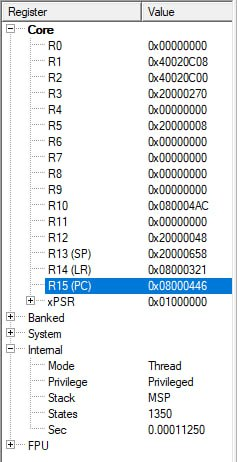
\includegraphics[width=0.50\textwidth]{reg1.jpg}
    \caption{Перша ітерація}
\end{figure}


\begin{figure}[H]
    \centering
    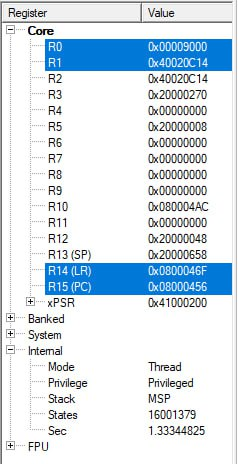
\includegraphics[width=0.50\textwidth]{reg2.jpg}
    \caption{Друга ітерація}
\end{figure}

\begin{figure}[H]
    \centering
    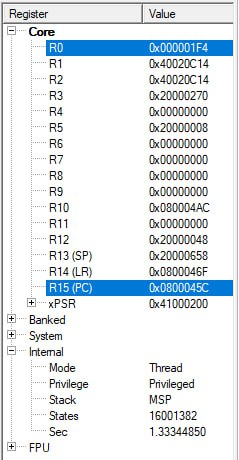
\includegraphics[width=0.50\textwidth]{reg3.jpg}
    \caption{Третя ітерація}
\end{figure}

\break
\paragraph{1.}Друга програма
\begin{verbatim}
    #include "stm32f4xx.h"   
    #include "stm32f4xx_gpio.h" 
    
    static GPIO_InitTypeDef gpio_a; 
    static GPIO_InitTypeDef gpio_d;
    
    int main(void) 
    {
    RCC_AHB1PeriphClockCmd(RCC_AHB1Periph_GPIOD | RCC_AHB1Periph_GPIOA,ENABLE);
     
    GPIO_StructInit(&gpio_a); 
    gpio_a.GPIO_Pin = GPIO_Pin_15; 
    gpio_a.GPIO_Mode = GPIO_Mode_IN;   
    GPIO_Init(GPIOA, &gpio_a);  	
        
    GPIO_StructInit(&gpio_d); 
    gpio_d.GPIO_Pin = GPIO_Pin_5; 
    gpio_d.GPIO_Mode = GPIO_Mode_OUT;   
    GPIO_Init(GPIOD, &gpio_d); 
        
     
      while (1) 
      {
        if(GPIO_ReadInputDataBit(GPIOA,GPIO_Pin_15) == 0)
        {
           GPIO_SetBits(GPIOD,GPIO_Pin_5);
           }
        else
        {
           GPIO_ResetBits(GPIOD,GPIO_Pin_5);
        }
      }
    }
    
    
\end{verbatim}
\begin{figure}[H]
    \centering
    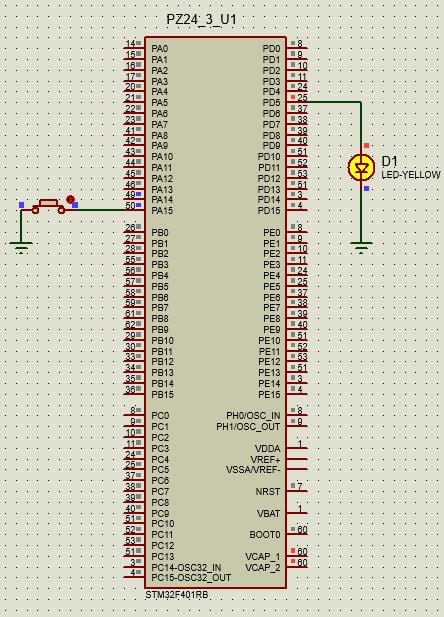
\includegraphics[width=0.90\textwidth]{smt32.jpg}
    \caption{Мікроконтроллер}
\end{figure}

\vspace{12pt}

\subsection*{Висновок} 
під час виконання лабораторної я успішно оволодів навичками роботи з цифровими портами мікроконтролера STM32F401RB. Вивчив основи програмування цифрових портів, розробив програму мовою C  в середовищі Keil μVision та змоделював її працездатність в системі Proteus.

\end{document}